\chapter{State-of-the-Art} \label{chap:sota}

\section*{}

In this chapter we will begin by making a more in depth presentation of the
process of gene expression. This will be followed by a literature and state of
the art review in the fields of \trans{} assembly and data mining.
Lastly, we will present some of the tools used in each of those areas and
common result evaluation techniques, as well as some relevant data
representation formats for genetic information.

\section{Biological Base Concepts}

Before dwelling in the details of the state of the art that are on the
foundation of the thesis, it is important to explain some concepts of the
domain of molecular biology. As explained in Chapter \ref{chap:intro}, gene
expression is the mechanism by which an organism's \dna{} can be expressed into
functional genetic products, like proteins. This process starts with the
genetic code, or nucleotide sequence, of each gene. Different genes in an
organism's \dna{} are responsible for the creation of different genetic
products. The process of gene expression itself is composed by two main stages,
transcription and translation \cite{leic:gene_expr}.

Transcription is the stage at which genetic data in the form of \dna{} is used
to synthesize \rna{}, being this the process that concerns the thesis' main
question. Several different types of \rna{} are produced by this process,
including mRNA (which specifies the sequences of amino acids that form a
protein), rRNA and tRNA, both later used in the translation stage. Simplifying
a gene's structure, it can be seen as composed by two types of sequences,
introns and exons, as seen in Figure \ref{fig:intron_exon}.

\begin{figure}[!htb]
  \begin{center}
    \leavevmode
    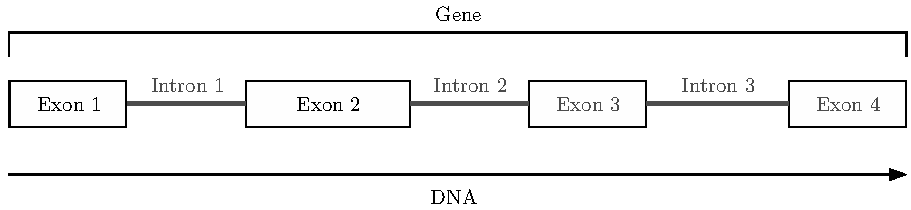
\includegraphics[width=1.0\textwidth]{intron_exon2}
    \caption[Overall structure of a gene]{Overall structure of a gene, with its
    different areas (simplified).}
    \label{fig:intron_exon}
  \end{center}
\end{figure}

Only the exons are useful in the gene expression process, being also known as
coding regions. Introns, on the other hand, are not used in the process. They
are present in an early stage mRNA molecule, the precursor mRNA, but are later
removed (or spliced) in the final molecule before the translation stage
\cite{leic:gene_expr}. Figure \ref{fig:splicing} illustrates the removal of
introns from the mRNA molecule, during the  splicing process. As stated before,
the main goal of this thesis is to explain how the final nucleotide sequence of
each exon affects the transcription speed of the exon itself.

\begin{figure}[!htb]
  \begin{center}
    \leavevmode
    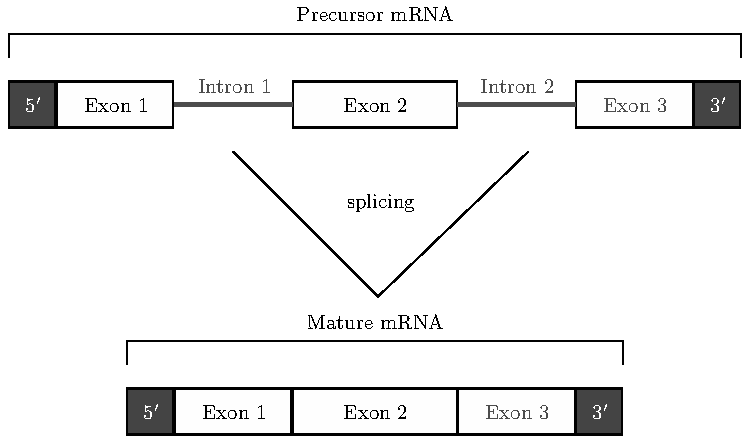
\includegraphics{splicing2}
    \caption[Removal of introns from precursor mRNA]{The removal (splicing) of
    introns from the precursor mRNA, during the transcription process.}
    \label{fig:splicing}
  \end{center}
\end{figure}

After the conclusion of the transcription process comes the translation process.
In this process, the synthesized mRNA is used to specify the sequence of amino
acids that constitute the particular protein being produced. The other types of
RNA molecules (rRNA and tRNA) are also used in this stage of the gene expression
process.

Obtaining this genetic information is done experimentally, by employing a
sequencing technique. For quite some time this process was carried out using
the Sanger's and other similar sequencing methods methods
\cite{Reis-Filho2009}. Though effective, such methods were notably slow and
costly, with large projects like the Human Genome Project (HGP) consuming
roughly thirteen years and US\$ 3 billion. These limitations were so severe
that, other than the realm of human genetics, this kind of study was restricted
to model organisms, such as the fruit fly and mouse genomes \cite{Wolf2013}.
The past few years have seen the appearance and rise in popularity of the
\ngs{} techniques. These techniques differ from the more classical ones by
producing larger amounts of information, at less cost. They are also typically
more cost effective than previous techniques and can be easily employed by
single laboratories, which has greatly contributed to their popularity. As a
disadvantage, \ngs{} techniques produce shorter reads than their older
counterparts, being that \qt{\textit{(...) transcriptome assembly from billions
of RNA-Seq reads (...) poses a significant informatics challenge}} \cite[p.
671]{Martin2011}. Although the thesis will not deal with the problems of
sequencing techniques, it is important to indicate that the read dataset that
will be used is the result of \ngs{} techniques. As such, we will use assembly
techniques more suited to situations where short reads are available.

\section{\rnaseq{} and \Trans{} Assembly}\label{sec:assembly}

\Trans{} assembly is the process by which experimentally obtained genetic data
reads can be organized and merged together in a partial or complete genome
expression profile. As stated above, the advent of next generation sequencing
techniques, with their reduced costs, greatly increased the availability of
genome sequencing data.

For years, microarrays were the standard tool available for examining features
of the transcriptome and global patterns of gene expression \cite{Wolf2013}.
However, microarrays are typically more oriented towards assembly against
existing reference data, hence limiting its application to species with well
known reference genomes. This is impractical, as \ngs{} techniques allow to
cheaply obtain genetic information of previously non-studied species. This is
one of the reasons that led to the inception of RNA-Seq. Contrary to
microarrays, RNA-Seq techniques are able to wield results that are suitable for
both reference guided assembly and \textit{de novo} assembly approaches
\cite{Wilhelm2009}. \textit{De novo} or exploratory assembly has captured the
interest of researchers in the past few years, leading to the appearance of
multiple RNA-Seq tools that are capable of making this type of assembly without
a reference genome \cite{nuno11:assemblathon}. Despite this amazing capability,
we will restrict this project to reference genome guided problems, which are
simpler and more suitable for a Masters level thesis.

\subsection{\rnaseq{} Tools}\label{sec:seqtools}

Below we will present some bioinformatic tools, used to support the multiple
steps of the \rnaseq{} process. Although there are several tools capable of
executing all steps of this process, it has been decided we will create our own
alignment/assembly pipeline, using specialized tools for every step. We will also present
some of the most popular file formats used in this context, along with some
tools used to manipulate those formats. We will focus in open source, Unix
command line based tools.

\subsubsection*{Tuxedo Suite}

The Tuxedo suite is a free, open-source collection of applications that has been
widely adopted as analysis toolset for fast alignment of short reads. It is
composed by four separate tools, Bowtie, TopHat, Cufflinks and CummRbund,
briefly reviewed below. These tools are extensively used for \rnaseq{} analysis.
Although the applications are made for command line execution, there are several
workflow managers, like Galaxy\footnote{\url{http://galaxyproject.org/}}, that
easily integrates with the suite, providing a web interface for its use.

\paragraph{Bowtie}

Bowtie\footnote{\url{http://bowtie-bio.sourceforge.net/index.shtml}} is an
ultrafast, memory-efficient short read aligner. Bowtie is typically used to
build a reference index for the genome of the organism being studied, for
posterior use by other tools, like TopHat. It can also output alignments in the
standard SAM format, allowing Bowtie to interoperate with tools like SAM Tools.
However, it should not be used as a general purpose alignment tool, as it was
created and is more effective when aligning short read sequences against large
reference genomes.

\paragraph{TopHat}

TopHat\footnote{\url{http://tophat.cbcb.umd.edu/}} is a fast splice junction
mapper for \rnaseq{} reads. It uses Bowtie as the underlying alignment tool,
using its results and a FASTA formated reference genome to identify splice
junctions between exons.

\paragraph{Cufflinks}

Cufflinks\footnote{\url{http://cufflinks.cbcb.umd.edu/}} assembles transcripts,
estimates their abundances, and tests for differential expression and regulation
in \rnaseq{} samples. It uses the SAM or BAM formatted files as input, typically
the ones produced by TopHat, outputting GTF files as a result.

\paragraph{CummeRbund}

Lastly, CummeRbund\footnote{\url{http://compbio.mit.edu/cummeRbund/}} is an R
package (see Section \ref{sec:mintools}) designed to help the visualization and
analysis of Cufflinks' \rnaseq{} output. As such, it is not directly involved in
the trascriptome alignment process. It takes the various output files from
Cufflinks and uses them to build a SQLite database describing appropriate
relationships between genes, transcripts, etc. It implements several plotting
functions, as well as commonly used data visualizations.

\subsubsection*{SAM Tools}

SAM Tools\footnote{\url{http://samtools.sourceforge.net/}} is a library 
package designed for parsing and manipulating alignment files in the SAM/BAM
format \cite{Li2009} (see Section \ref{sec:formats}). SAM Tools has two separate
implementations, one in C and the other in Java, with slightly different
functionality. Beyond manipulation of SAM and BAM files, this package is able to
convert between other read alignment formats, sort and merge alignments and show
them in a text-based viewer.

\subsubsection*{BLAST}

BLAST\footnote{\url{http://blast.ncbi.nlm.nih.gov/Blast.cgi}} is a tool,
implemented in C++, that is used to find regions of local similarity between
biological sequences. It uses FASTA sequences (see Section \ref{sec:formats}) as
search input and outputs the results reports in XML, HTML or plain text. There
are several different BLAST programs available at the moment, that can be used
depending on our objective and type of data. BLAST is particularly useful to
search biologic sequence databases, but can be used for other purposes, like
identifying an unknown species or comparing common genes in two related
species.

\subsection{Relevant Standard File Formats}\label{sec:formats}

As expected, the great diversity of \rnaseq{} tools brings with it a wealth of
file formats. Some of these formats are developed from the ground up to satisfy
a specific need, while other are mere contextual adaptations or specializations
of already established formats. Below we will present a few of the most popular
and widely spread file formats, talking about their basic structure, the types
of data they represent and their applications.

\subsubsection*{FASTA}

FASTA is the standard line and character sequence format used by NCBI
\cite{ncbi:fasta}, using this last organization's character code conventions. It
is a simple format, that can be used to easily store data represented by
character sequences, like nucleotide (\dna, \rna) or amino acid (protein)
sequences. This file format is widely use to store sequencing reads, \dna/\rna{}
sequences and other character sequences in database systems. Its simplicity
makes it extremely easy to manipulate and parse, presenting also an attractive
solution for data transfer between different tools.

\subsubsection*{FASTQ}

FASTQ is used to store store character sequences, typically nucleotide sequences
\cite{Cock2010}. It is quite similar to the standard FASTA format, in respect to
the manner in which character sequences are represented. However, for every
sequence, there is a second sequence of equal length, representing the quality
scores of the original sequence. These quality scores are also represented as
single characters, taking values between and including ASCII-33 to ASCII-126.
It is typically used in the same situations as the FASTA format, when quality
scores are available/relevant.

\subsubsection*{SAM and BAM}

The SAM format is a text format for storing sequence alignment data
\cite{genome:sam}. It is widely used to store mapping information between
sequencing reads and a given reference genome. This sort of information is
typically the product of sequencing alignment tools, that consume sequencing
reads from FASTQ files and align them with a reference genome.

The BAM format contains exactly the same information as the SAM format and the
same rules apply for both formats. The difference between both formats lies in
their encoding. While SAM is a text based format, BAM is a binary format. This
means that BAM sacrifices human readability for increased machine processing
performance, as it is more efficient to work with compressed and indexed binary
data.

\subsubsection*{VCF}

VCF is a text file format used to store gene sequence variants \cite{smith13}.
In the past few years, as larger and larger genome sequencing projects became
more common (like the 1000 Genomes Project\footnote{The 1000 Genomes Project,
started back in 2008, is an international effort to establish the most
comprehensive catalogue to date of human genetic variations.}), storing such
large amounts of information became a serious concern. To address these concerns
the VCF format was created. Instead of storing the complete genome, VCF stores
only the variations (and their respective positions) of newly sequenced genomes
relatively to a known reference genome, typically in a compressed text file. As
such, it is a format often used when building genome databases.

\subsubsection*{GFF and GTF}

GFF is a text based file format to store gene features \cite{sanger11}. Many
genome assembly tools execute this process in two separate steps: feature
detection for identification of specific regions (exons, introns, etc.) and
genome assembly, using those features as reference. However, often times it is
beneficial to decouple these two steps, using different and more efficient tools
for each. As such, the GFF format emerged as a protocol for feature information
transfer between tools.

The GTF format is similar to the GFF format, in which it is based. It is also
used in similar situations. However, GTF builds on top of GFF, defining
additional conventions, specific to the domain of genetic information. Despite
their initial relation, both formats continue to be developed individually.

\section{Data Mining}\label{sec:mlearning}

Data mining is the process of \qt{\textit{extracting or \qt{mining} knowledge
from large amounts of data}} \cite[p. 5]{han2006data}. As such, it consists of a
set of techniques that can be used to find interesting patterns in large data
sets, that translate in newfound knowledge. Data mining borrows techniques from
multiple fields, such as artificial intelligence, machine learning, statistics,
and database systems \cite{Chakrabarti2012}. Its ultimate goal is to combine all
those techniques and transform large and (apparently) meaningless sets of data
into understandable and useful information. Thus, data mining was motivated by
the perspective of harnessing the abundance of data, that characterizes today's
information systems, to produce meaningful knowledge.

Because of their large quantities of input data, data mining tasks are usually
totally, or at least partially, automated. As such, there are several algorithms
for these tasks and tools that implements such algorithms, as presented in
Section \ref{sec:minalgo} and Section \ref{sec:mintools}, respectively.

We can divide data mining into main types: descriptive data mining and
predictive data mining \cite{Fayyad1996}. Descriptive data mining is focused on
finding the underlying structure of a given set of data. Instead of predicting
future values, it concerns the intrinsic structure, relations and
interconnectedness of the data being analyzed, presenting its interesting
characteristics without having any predefined target. On the other hand,
predictive data mining is used to predict explicit values, based on patterns
determined from the dataset. With predictive data mining we try to build models
using known data and use those models as a base to predict future behavior.

As we're seeing, data mining does not represent a single type problem. In fact
there are several different types of problems that can be addressed by data
mining techniques. Each of these problems may require a different data mining
method. A brief review of the most common methods is given below.

\begin{description}

  \item[Classification]
  is a method that tries to generalize the already known structure of a
  dataset, so that it applies to new datasets. In other words, with
  classification we try to learn a function that is capable of mapping our data
  into predefined classes.

  \item[Regression]
  tries to learn a function that models relationships between variables in the
  dataset. That function can latter be used to find real value predictions of
  future behavior of the same or similar datasets.

  \item[Clustering]
  consists in identifying a finite set of categories or clusters of similar
  values, to describe the dataset. As such, it is used without prior knowledge
  about data structure.

  \item[Summarization]
  provides a more compact representation of a subset of data, in a way that the
  summarized data retains the central points of the original data. This can be
  accomplished in several different ways, like using report generation or
  multivariate visualization techniques.

  \item[Dependency modeling]
  finds a model which describes relationships between variables, revealing their
  dependencies.

  \item[Change and deviation detection]
  tries to discover the most significant changes in the data, when compared with
  previously measured data. This method is useful to find interesting data
  variations or data errors.

\end{description}

\subsection{Data Mining Algorithms}\label{sec:minalgo}

In this project we will be concerned with the classification side of data
mining. Below, we will review some algorithms that can be used in
classification problems.

%\subsubsection*{Decision Trees}

%\textit{\qt{A decision tree is a flowchart-like tree structure, where each
%internal node (nonleaf node) denotes a test on an attribute, each branch
%represents an outcome of the test, and each leaf node (or terminal node) holds a
%class label}} \cite[p. 291]{han2006data}, as seen in Figure \ref{fig:tree}.
%Decision tree learning algorithms use a decision tree as a predictive model,
%that maps observed data about an individual to conclusions about the expected
%value for that individual. From a classification problem standpoint, this means
%means creating a decision tree structure that is able to predict the class of an
%individual based on its attributes.

%\begin{figure}[htb]
  %\centering

  %% Node levels and identation.
  %\tikzstyle{level 1}=[level distance=1.5cm, sibling distance=4.25cm]
  %\tikzstyle{level 2}=[level distance=1.5cm, sibling distance=2.25cm]
  %\tikzstyle{level 3}=[level distance=1.5cm, sibling distance=4.25cm]
  %\tikzstyle{level 4}=[level distance=1.5cm, sibling distance=2.25cm]

  %% Node style.
  %\tikzset{decision/.style={
    %draw=black!80, solid, fill=white!10, rectangle,
    %anchor=north,
    %inner sep=2mm, outer sep=0, text centered, growth parent anchor=south}
  %}
  %\tikzset{prediction/.style={
    %draw=black!80, solid, fill=white!30, ellipse,
    %anchor=north,
    %inner sep=2mm, outer sep=0, text centered, growth parent anchor=south,
    %minimum height=1cm,minimum width=1.3cm}
  %}

  %% Tree.
  %\begin{tikzpicture}
    %\node [decision] {\textit{age?}} [solid, -latex, thick, -]
      %child {
        %node [decision] {\textit{student?}} [solid, -latex, thick, -]
        %child {
          %node [prediction] {no} [solid, -latex, thick, -]
          %edge from parent
          %node[left] {no}
        %}
        %child {
          %node [prediction] {yes} [solid, -latex, thick, -]
          %edge from parent
          %node[right] {yes}
        %}
        %edge from parent
        %node[above left] {youth}
      %}
      %child {
        %node [prediction] {yes} [solid, -latex, thick, -]
        %edge from parent
        %node[below,fill=white,inner sep=1pt] {middle\_aged}
      %}
      %child {
        %node [decision] {\textit{credit\_rating?}} [solid, -latex, thick, -]
        %child {
          %node [prediction] {no} [solid, -latex, thick, -]
          %edge from parent
          %node[left] {no}
        %}
        %child {
          %node [prediction] {yes} [solid, -latex, thick, -]
          %edge from parent
          %node[right] {yes}
        %}
        %edge from parent
        %node[above right] {senior}
      %}
    %;
  %\end{tikzpicture}
  %\caption[Example of a decision tree]
  %{Example of a decision tree for the concept \textit{buys\_computer},
  %indicating whether a customer is likely to purchase a computer. Each internal
  %(nonleaf) node represents a test on an attribute. Each leaf node represents a
  %class (either \textit{buys\_computer = yes} or \textit{buys\_computer = no})
  %\cite[p. 291]{han2006data}.}
  %\label{fig:tree}
%\end{figure}

%Decision tree classifiers are among the most popular used nowadays. They are
%able to handle high dimensional data and their learning and classification steps
%are simple and fast. Other than that, the construction of decision tree
%classifiers does not not require domain knowledge or parameter setting. These
%classifiers usually have a good level of accuracy, though it may vary with the
%type of data available.

%That are several algorithms that use the decision tree principle, most notably
%\textit{ID3}, \textit{C4.5} and \textit{CART}. As the problem of learning an
%optimal decision tree is NP-complete, most algorithms for decision tree
%construction are based in some sort of heuristics (the aforementioned algorithms
%adopt a greedy approach).

%\subsubsection*{Random Forest}

%Random forest \cite{breiman2001random} is an ensemble approach for
%classification and regression problems. Ensembles use a divide-and-conquer
%approach to classification problems, in order to increase performance. The base
%principle behind ensembles is simple: a group of \qt{weak} learners can come
%together to become a \qt{strong} learner, where their individual shortcomings
%are amortized by their combined results. As such, random forest algorithms use
%several individual decision trees, in order to mitigate the problems with
%variance and bias in single decision trees.

%Each individual tree in the forest in trained used a random subset of the
%original dataset, where the subsets distribution is the same across the forest.
%Then, at each node we choose the predictor variable that provides the best split
%(as per an objective function) and use it to do a binary split at that node.
%This continues until all the trees are grown to the largest extent possible, as
%no pruning is made.

%Random forest is a fairly fast method and is able to deal with unbalanced and
%missing data. It as few parameters to tune and can be easily and effectively
%used with default parameters. As a limitation, when used for regression random
%forests cannot predict beyond the range in the training data, and that they may
%overfit datasets that are particularly noisy.

%\subsubsection*{Support Vector Machines}

%Support vector machines are a set of related supervised learning methods used
%for pattern recognition, that can be applied to classification and regression
%problems \cite{Cortes1995}. SVMs typically fall under a simple premise, the
%spacial division of classes. As seen in Figure \ref{fig:svm}, we can define an
%infinite number of possible separating hyperplanes or \qt{decision boundaries}
%(in this case straight lines). The objective of an SVM is to find the optimal
%hyperplane or set of hyperplanes to separate the classes. To classify a new set
%of data each value is represented in the space and classified according to the
%side of the hyperplane in which it falls.

%\begin{figure}[!htb]
  %\begin{center}
    %\leavevmode
    %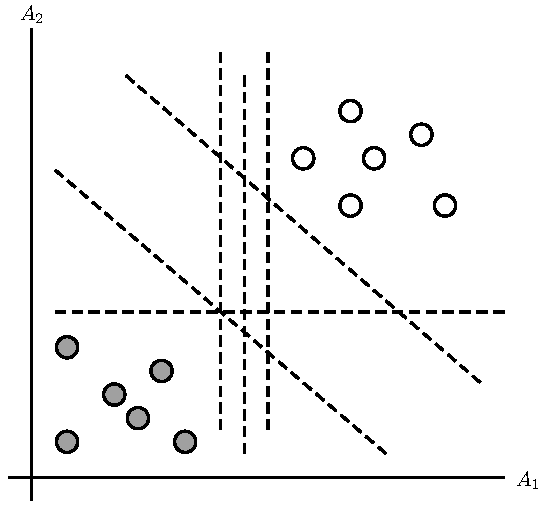
\includegraphics[width=0.6\textwidth]{svm2}
    %\caption[Example of linearly separable training data]
    %{Example of linearly separable training data in a two dimensional
    %space. There are an infinite number of (possible) separating hyperplanes or
    %\qt{decision boundaries} \cite[p. 338]{han2006data}.}
    %\label{fig:svm}
  %\end{center}
%\end{figure}

%SVMs are widely used nowadays, and have been successfully applied in areas such
%handwritten digit recognition, object recognition, and speaker identification,
%as well as benchmark time-series prediction tests \cite{han2006data}. They are
%typically regarded. They are highly accurate, due in part to their ability to
%model complex nonlinear decision boundaries.

%However, even the fastest SVMs can be extremely slow in both the training and
%testing steps. It is also directly limited to two-class tasks, requiring the use
%of other algorithms to reduce multi-class tasks to binary ones.

%\subsubsection*{K-NN}

%K-NN is a non-parametric method for classification and regression problems.
%First described in the early 1950s \cite{han2006data}, it is one of the simplest
%machine learning algorithms and is widely used in the area of pattern
%recognition.

%Nearest neighbor classifiers are based on the premise of learning by analogy, in
%other words, by comparing a given test tuple with similar training tuples. This
%classification of tuples as \qt{similar} is typically based on simple rules,
%like the \textit{Euclidean distance} between tuples.

%In k-NN, each training tuple is described by $n$ attributes and is represented
%as a point in an $n$-dimensional space. For classification problems, the test
%tuple is represented in this space, along with the training tuples. The unknown
%tuple is then assigned to the most common class among its $k$ nearest neighbors.

%K-NN as several advantages when compared to other classification algorithms. For
%one it has a very simple implementation. it is also very robust in terms of
%search space (the classes don't have to be linearly separable) and has few
%parameters, making it easy to tune. On the other side, it is an expensive method
%in terms of testing, as we need to calculate the distance between a testing
%tuple and every other known tuple. Furthermore, it is sensitive to noisy or
%irrelevant attributes and unbalanced datasets.

\subsubsection*{Inductive Logic Programming}

ILP is a subfield of machine learning that uses first order logic to represent
both data and models \cite{Lavrac1998}. ILP induces hypotheses (models) from
examples and background knowledge. Examples are of two types: instances of the
concept to be \qt{learned} and non-instances of the concept. Background
knowledge is a set of predicates encoding all information that the experts find
useful to construct the models. ILP might be used to tackle several machine
learning and data mining problems, like classification, regression and
clustering.

The first and most important motivation for ILP systems is that they overcome
the representation limitations of attribute-value learning systems, such as the
previously mentioned data mining algorithms. Attribute-value systems base their
representations of data in table based representations. Although effective in
many situations, these representation is not very expressive and might not even
be feasible for certain problems \cite{Bratko:1995:AIL:219717.219771}. The
second motivation for ILP is that by using a logical representation, the
hypotheses are understandable and interpretable by humans, being therefore
useful to explain the phenomenons that produce the data. This representation
also means that background knowledge can be represented and employed in the
induction process, in contrast to attribute-value models, where this information
is difficult to represent.

Despite these advantages, ILP cannot be applied indiscriminately to any
classification or regression problem. ILP systems are typically very heavy when
it comes to computational resource consumption and run for long periods of time
\cite{fonseca2003implementation}.

%\subsection{Model Evaluation Procedures and Measures}\label{sec:mineval}

%Creating a data model using a suitable classification algorithms is not the last
%step in the data mining process. At this point our model works well with the
%original training data, but we need to verify its power to generalize to other
%sets of data. Without this evaluation process, our models may be susceptible to
%problems like overfitting, in which the model wrongly describes a random error
%or data noise as a significant pattern \cite{han2006data}. As such, we need
%methods that allow us to test our models before deployment, as well as standard
%measures, to determine their quality.

%\subsubsection*{Evaluation Procedures}

%As stated, evaluation procedures are essential to verify the generalization
%capabilities of a given model. These procedures typically consist of dividing
%the test dataset in two or more subsets, using some of them for training and the
%others for testing. We will present a brief overview of some of these procedures
%below.

%\paragraph{Hold-Out}

%The \textit{hold-out} method reserves a part of the dataset for training
%purposes and uses the remaining data for testing \cite{witten2011data}.
%Typically we separate one third of the original dataset for testing, using the
%other two thirds for training.

%However, this arbitrary division of the dataset might be problematic if the
%subsets aren't representative of the population. For example, if the test subset
%is missing a class our results might be erratic. One way to attenuate this
%problem is to use stratification. Using stratification of the dataset we ensure
%that both subsets are representative, with approximately equal proportions for
%each class. We can lessen error rates even further and make the
%\textit{hold-out} estimate more reliable using the \textit{repeated hold-out}
%method. This is an iterative method, where in each iteration a subset is
%randomly selected to use as training (possibly using set stratification), using
%the remaining subset for testing. After all the iterations, the error rates of
%each one are averaged to yield an overall error rate.

%\paragraph{Cross-Validation}

%\textit{Repeated hold-out} methods pose a problem: the different test subsets
%will eventually overlap. This may cause that some examples never appear in the
%training subsets. The overlapping problem can be solved using the
%\textit{cross-validation} procedure, also called \textit{k-fold
%cross-validation}. This method consists in splitting the original dataset into
%\textit{k} subsets, using each subset in turn for testing and the remainder for
%training.

%The standard method for evaluation is \textit{10-fold cross validation}, where
%the dataset is divided into ten subsets. The subsets are typically stratified to
%reduce result variance. In each iteration one of the ten folds is picked as test
%and the other nine are used for training. Sometimes, to further reduce variance,
%\textit{repeated stratified cross-validation} is used, repeating normal
%\textit{10-fold cross-validation} ten times, then averaging the results.

%\paragraph{Leave-One-Out}

%\textit{Leave-one-out} method is a form of \textit{cross-validation}, taken to
%extreme lengths. In this particular method, the original dataset is divided into
%\textit{n} folds, where \textit{n} is the number is the number of individual
%training instances. It has some benefits, like allowing for a better use of the
%dataset and involving no random set sampling. However, the sheer number of folds
%and tests makes it a very computationally expensive method. Another disadvantage
%is that no stratification is possible, as there is always only one instance in
%the test subset.

%\subsubsection*{Common Measures}

%Applying evaluation procedures is not sufficient by itself. In order to appraise
%the quality of our models, we need to use standard quality measures, that give
%meaning to the obtained results. Below we will review some common measures, used
%in the context of classification problems.

%\paragraph{Precision}

%Precision determines the fraction of positive cases that are correctly
%identified as such. Low precision values mean that the model identifies many
%cases as positive when they are in reality false positives. Precision is
%calculated as shown in Equation \ref{eq:precision}.

%\begin{equation}
  %Precision=\frac{\tp}{\tp + \fp}
  %\label{eq:precision}
%\end{equation}

%\paragraph{Recall}

%Recall represents the portion of actual positive results in the dataset that
%were identified as such. From a statistical standpoint, it can be viewed as the
%average probability of find all the positive cases in the dataset. The value is
%computed using Equation \ref{eq:recall}.

%\begin{equation}
  %Recall=\frac{\tp}{\tp + \fn}
  %\label{eq:recall}
%\end{equation}

%\paragraph{Accuracy}

%Accuracy represents the percentage of predictions that are in fact correct. This
%measure relates to the ability of our model to correctly predict the class of
%new data. It can be calculated with Equation \ref{eq:accuracy}. For a given
%problem, better accuracy might not always mean that a model is better than
%another. As such, other measures like precision and recall are also taken into
%account.

%\begin{equation}
  %Accuracy=\frac{\tp + \tn}{\tp + \fp + \tn + \fn}
  %\label{eq:accuracy}
%\end{equation}

%\paragraph{F-Measure}

%F-measure is the harmonic mean of precision and recall. The reason behind the
%usage of an harmonic mean instead of an arithmetic mean is that the first is
%more intuitive, when computing a mean of ratios \cite{Sasaki2007}. F-measure is
%calculated as shown in Equation \ref{eq:fmeasure}. It is particularly useful to
%differentiate between cases where one of the variables (precision or recall) has
%a very high value and the other has a very low value. For example, if in a
%particular situation we have a precision of $1.0$ and a recall of $0.2$, the
%arithmetic mean would be $0.6$. However, a system with a recall as low as $0.2$
%might not be very useful. On the other hand, in the same situation the harmonic
%mean would be $0.333(3)$, giving a much more realistic measure of the quality of
%the model.

%\begin{equation}
  %\textit{F-measure}=2 \cdot \frac{\mathit{Precision} \cdot
  %\mathit{Recall}}{\mathit{Precision}+\mathit{Recall}} \label{eq:fmeasure}
%\end{equation}

%\paragraph{AUC}

%Sometimes in order to evaluate the quality of a certain model we might plot a
%ROC (or \textit{receiver operating characteristic}) curve. ROC curves depict the
%performance of a classifier without regard to class distribution or error
%costs. The curve is build by plotting false positive rates in the $x$ axis and
%true positive rates (recalls) in the $y$ axis (Figure \ref{fig:roccurve}).

%\begin{figure}[ht]
  %\begin{center}
    %\begin{tikzpicture}
      %\begin{axis}[
        %domain=0:1,
        %legend pos=south east,
        %xlabel=False Positive Rate,
        %ylabel=True Positive Rate]
        %\addplot[mark=none, samples=10, red] function {x};
        %\addplot[smooth, color=blue, mark=none]
          %plot coordinates {
              %(0.0,0.0)
              %(0.1,0.4)
              %(0.2,0.7)
              %(0.3,0.8)
              %(0.4,0.85)
              %(0.5,0.88)
              %(0.6,0.91)
              %(0.7,0.94)
              %(0.8,0.97)
              %(0.9,0.99)
              %(1.0,1.0)
          %};
        %\legend{Random model,Created model}
      %\end{axis}
    %\end{tikzpicture}
    %\caption[Example of ROC curve]{Example of ROC curve.}
    %\label{fig:roccurve}
  %\end{center}
%\end{figure}

%However, the curve can be hard to interpret at times. In this situation we can
%use the AUC measure (or \textit{area under the curve}), in order to condensate
%the curve's information in a single value. The AUC of a random classification
%system is $0.5$. This means that any model that as an AUC of $0.5$ is not able
%to distinguish between two groups. As the AUC increases, the model's quality
%also increases and at a value of AUC equal to $1.0$ the model is able to
%perfectly separate both groups.

\subsection{Data Mining Tools}\label{sec:mintools}

Except in rare cases of very specific problems, it typically makes no sense for
someone to implement any data mining algorithm that they might need. In fact,
today we have lots of data mining tools (many of which are free), that already
implement many of those algorithms. These tools are usually customizable, making
it easy to adapt them to most problems. Below we'll briefly review some of the
most popular data mining tools, that apply to the specific needs of this thesis.

\subsubsection*{RapidMiner}

RapidMiner\footnote{\url{http://www.rapidminer.com/}} is a complete solution for
data mining problems. it is available as a standalone GUI based application, as
seen in Figure \ref{fig:rapidminer}. It is a commercial application, although
its core and earlier versions are distributed under an open source license and
it offers a free version, beyond its multiple paid versions. Being one of the
most popular data mining tools used today, its applications span several
domains, including education, training, industrial and personal applications,
among others. Its functionality can also be easily extended through the use of
plugins\footnote{Plugin is a software module that adds new functionality to an
existing software application. Plugins are typically dependent on the platform
they extend and can't be used as standalone tools.}, reflecting in an increased
value for this tool. One such example in the area of bioinformatics is the
integration plugin between RapidMiner and the
Taverna\footnote{\url{http://www.taverna.org.uk/}} open source workflow
management system \cite{Jupp2011}.

\begin{figure}[!htb]
  \begin{center}
    \leavevmode
    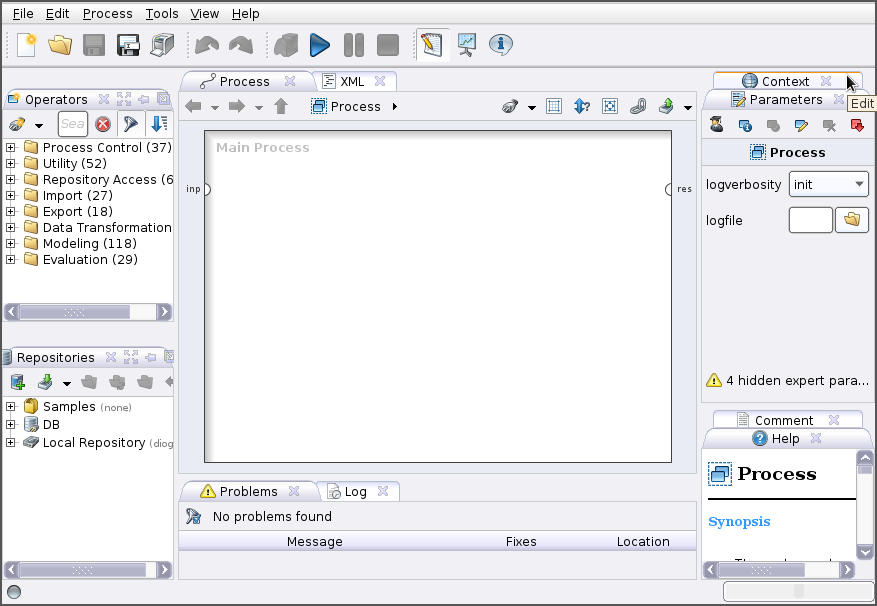
\includegraphics[width=1.0\textwidth]{rapidminer}
    \caption[RapidMiner user interface]{RapidMiner user interface.}
    \label{fig:rapidminer}
  \end{center}
\end{figure}

\subsubsection*{Weka}

Weka\footnote{\url{http://www.cs.waikato.ac.nz/ml/weka/}} is an open source tool that
collects several machine learning algorithms and allows its user to easily apply
those algorithms to data mining tasks \cite{Hall}. Created at the University of
Waikato, New Zeland in 1997 (the current version was completely rewritten in
1997, despite the first iteration of the tool being developed as early as 1993),
it is still in active development to date. Weka supports several common data
mining tasks, like data preprocessing, classification, clustering, regression
and data visualization. it is core libraries are written in Java and allow for an
easy integration of its data mining algorithms in pre existing code and
applications. Other than that, Weka can be used directly through a command
line/terminal or through one of its multiple GUIs (Figure \ref{fig:weka}). Its
simple API and well structure architecture allow it to be easily extended by
users, should they need new functionalities.

\begin{figure}[!htb]
  \begin{center}
    \leavevmode
    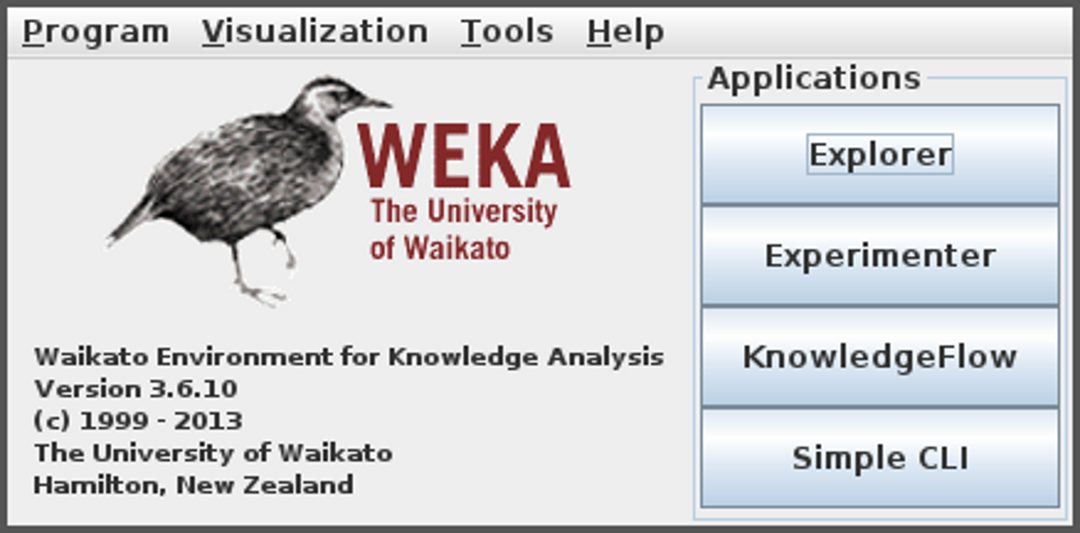
\includegraphics[width=0.7\textwidth]{weka}
    \caption[Weka interface selection]{Weka interface selection.}
    \label{fig:weka}
  \end{center}
\end{figure}

\subsubsection*{R Language}

R\footnote{\url{http://www.r-project.org/}} is a free programming language and
software environment for statistical computing and graphics generation.
Originally developed by Ross Ihaka and Robert Gentleman at the University of
Auckland, New Zealand in 1993 \cite{Ihaka1998}, it is still under active
development. R is typically used by statisticians and data miners, either for
direct data analysis or for developing new statistical software \cite{Fox2005}.

R is an implementation of the S programming language\footnote{S is an object
oriented statistical programming language, appearing in 1976 at Bell
Laboratories.}, borrowing some characteristics from the Scheme programming
language. it is core is written in a combination of C, Fortran and R itself. It
is possible directly manipulate R objects in languages like C, C++ and Java. R
can be used directly through the command line or through several third party
graphical user interfaces like
Deducer\footnote{\url{http://www.deducer.org/pmwiki/index.php}}. There are also
R wrappers for several scripting languages.

R provides several different statistical and graphical techniques, including
linear and nonlinear modeling, classical statistical tests, time-series
analysis, classification, clustering, among others. It can also be used to
produce publication-quality static graphics. Tools like Sweave
\cite{lmucs-papers:Leisch:2002} allow users to embed R code in \LaTeX{}
documents, for complete data analysis.

\paragraph{Bioconductor Package}

Bioconductor is a free and open source set of tools for genomic data analysis,
in the context of molecular biology \cite{lmucs-papers:Leisch:2002}. It is
primarily based on R. It is under active development, with two stable releases
each year. Counting with more than seven hundred different packages, it is the
most comprehensive set of genomic data analysis tools available for the R
programming language. It also provides a set of tools to read and manipulate
several of the most common file formats used in molecular biology oriented
applications, including FASTA, FASTQ, BAM and GFF.

\section{Chapter Conclusions}

In this chapter we gave a brief introduction of the molecular biology concepts
that serve as base of the thesis. We also reviewed the concepts on RNA-Seq and
data mining and presented short analyses of concrete tools that will likely be
used during the project.

At this moment we do not possess all the necessary information about the dataset
that will be used in the data mining phase of the project. We are unable, at the
present, to determine the nature of our data, which means that we cannot predict
whether it could be modeled by classification algorithms. As such, we presented
ILP as an alternative approach for this situation. In case ILP techniques become
in fact necessary, further work will include a more profound and complete
revision.
